\section{Methodology}

This section describes the methodology of the project in detail. The stages of
development from start to finish are explained, including strategies, design
choices, development lifecycles, and technological specifics.

The main goal of this project was to promote citizen science by building a platform
with an integrated machine learning model for birdwatchers and enthusiasts. The
project was divided into two separate phases. These phases consisted of the machine
learning phase of the project and the web platform development phase. The project
followed a structured methodology that combined a comparative analysis of different
machine learning models and applied software development.

The machine learning phase included algorithm selection, data collection, model
development, and evaluation. On the other hand, the web platform development phase
included the design and development of the website, integration of the machine
learning model, and testing.

\subsection{Machine Learning Model Development and Comparative Analysis}

The first main phase of the project was the development of machine learning models
for bird species identification. This phase included data acquisition,
preprocessing, model selection, training, and evaluation. The details of each step
are explained in the following subsections.

\subsubsection{Data Acquisition}

When developing a machine learning model, one of the most important requirements is
the availability of a large, high-quality dataset to train the models properly. In
this project, multiple models were evaluated, and high performance was expected from
them. To achieve accurate results, large numbers of bird images taken from different
angles were required. Furthermore, the data had to be labeled with the correct bird
species for the models to be trained effectively.

Because tens of thousands of bird images were required, it was not feasible to
create such a dataset manually. Instead, existing data was gathered. GBIF, which
stands for Global Biodiversity Information Facility, was used to construct the
dataset. It is an open-access biodiversity platform that collects species
observation records from various sources \cite{gbif2025}. These sources are mostly
citizen science platforms such as iNaturalist \cite{inaturalist2025} and
Observation.org \cite{observation2025}. This once again demonstrates the importance
of citizen science. A single organization would not be able to maintain records of
the increasing number of species from every part of the world. Alternatively,
citizens from around the world keep records of species around them by uploading
observations. As people use these platforms, massive datasets are created that would
be almost impossible for a single organization to construct independently.

In this project, GBIF was used to construct a dataset of bird images. In order to
limit the scope of the project, bird species that are commonly observed in Turkey
were selected. The species were selected with reference to observation counts in
Turkey \cite{ebird2025}. Initially, the constructed dataset included 23 bird
species commonly observed in Turkey. The dataset consisted of 5000 images for each
species and a total of 115000 images.

The metadata for the selected species was downloaded from GBIF. Only records that
included an image and reliable species labels were used. The data downloaded from
GBIF was compiled from many different sources and included metadata such as species
name, location of observation, datetime of observation, observer information,
observation license, life stage of the organism, and most importantly, multimedia
related to the observation.

For each selected bird species, the last ten thousand observations were downloaded
from GBIF. Then, using a Python script \cite{python2025}, the images were downloaded
into their respective folders in Google Drive \cite{googledrive2025}. A dataset
containing bird images labeled according to their species folders was constructed.
Sample images from the constructed dataset are shown in Figure
\ref{fig:bird_dataset_sample}.

\begin{figure}[H]
    \centering
    
\includegraphics[width=0.9\linewidth]{images/bird_dataset_sample.png}
    \caption{Sample images from the bird dataset with species labels}
    \label{fig:bird_dataset_sample}
\end{figure}

After completing the comparative analysis of different machine learning models using
the constructed dataset, further experiments were conducted using the best-performing
model. It was believed that the best-performing model would provide even better
results when trained on a larger dataset. Therefore, the dataset was later expanded
to include a total of 30 bird species. The final dataset included 150000 images,
with 5000 images for each species.

The bird species included in the final dataset are listed in Table
\ref{tab:bird_species_list}.

\begin{table}[H]
\centering
\caption{Bird species included in the final dataset}
\label{tab:bird_species_list}
\begin{tabular}{|c|l|l|}
\hline
\textbf{No} & \textbf{Common Name} & \textbf{Scientific Name} \\ \hline
1  & Yellow-legged Gull & \textit{Larus michahellis} \\ \hline
2  & Hooded Crow & \textit{Corvus cornix} \\ \hline
3  & Laughing Dove & \textit{Spilopelia senegalensis} \\ \hline
4  & Grey Heron & \textit{Ardea cinerea} \\ \hline
5  & Great Cormorant & \textit{Phalacrocorax carbo} \\ \hline
6  & Black-headed Gull & \textit{Chroicocephalus ridibundus} \\ \hline
7  & House Sparrow & \textit{Passer domesticus} \\ \hline
8  & Rose-ringed Parakeet & \textit{Psittacula krameri} \\ \hline
9  & European Shag & \textit{Gulosus aristotelis} \\ \hline
10 & Rock Pigeon & \textit{Columba livia} \\ \hline
11 & Common Myna & \textit{Acridotheres tristis} \\ \hline
12 & Common Starling & \textit{Sturnus vulgaris} \\ \hline
13 & Mallard & \textit{Anas platyrhynchos} \\ \hline
14 & Alexandrine Parakeet & \textit{Psittacula eupatria} \\ \hline
15 & Eurasian Jackdaw & \textit{Coloeus monedula} \\ \hline
16 & Great Tit & \textit{Parus major} \\ \hline
17 & Common Chaffinch & \textit{Fringilla coelebs} \\ \hline
18 & Pygmy Cormorant & \textit{Microcarbo pygmaeus} \\ \hline
19 & Eurasian Magpie & \textit{Pica pica} \\ \hline
20 & European Robin & \textit{Erithacus rubecula} \\ \hline
21 & Common Buzzard & \textit{Buteo buteo} \\ \hline
22 & Yelkouan Shearwater & \textit{Puffinus yelkouan} \\ \hline
23 & Alpine Swift & \textit{Tachymarptis melba} \\ \hline
24 & Eurasian Coot & \textit{Fulica atra} \\ \hline
25 & White Stork & \textit{Ciconia ciconia} \\ \hline
26 & White Wagtail & \textit{Motacilla alba} \\ \hline
27 & Eurasian Sparrowhawk & \textit{Accipiter nisus} \\ \hline
28 & Eurasian Blackbird & \textit{Turdus merula} \\ \hline
29 & Eurasian Jay & \textit{Garrulus glandarius} \\ \hline
30 & Eurasian Blue Tit & \textit{Cyanistes caeruleus} \\ \hline
\end{tabular}
\end{table}

\subsubsection{Data Preprocessing}

The collected image dataset was preprocessed to ensure that it was suitable for
training the machine learning models. Initially, low-quality and corrupted images
were removed from the dataset and replaced to keep class balance. The images were 
then resized to a consistent size to match the input dimensions required by the 
selected deep learning architectures.

To increase dataset variability and improve model generalization, several data
augmentation techniques were applied. These augmentations included random
rotations, horizontal flipping, brightness adjustments, and other minor
transformations. The purpose of these augmentations was to improve the robustness
of the models against variations commonly found in real-world bird photographs,
such as changes in lighting conditions, viewing angles, and image composition.

After preprocessing was completed, the dataset was divided into training,
validation, and testing subsets using a fixed splitting strategy. A total of
80\% of the dataset was reserved for training, while the remaining 20\% was
equally divided between validation and testing subsets.

\subsubsection{Model Selection}

During the literature review, studies related to bird species identification were
analyzed. In accordance with the findings obtained from the literature, model
selection in this project focused on deep learning architectures. Traditional
machine learning algorithms such as Support Vector Machines (SVMs) and Random
Forests generally underperform compared to deep learning models and are unable to
achieve the desired accuracy levels for fine-grained image classification tasks
\cite{lolge2025evolution}. Since this project focused on image-based bird species
classification, models that perform effectively on visual data were required.

This project focused on deep learning-based Convolutional Neural Network (CNN)
architectures that are widely used for image classification tasks. CNN-based
models are more suitable for identifying species from images because they are
capable of extracting complex hierarchical visual features such as texture,
shape, colour, and local patterns \cite{chen2024fetfgvc}. The following architectures
were selected because they frequently appear in the literature and have
demonstrated strong performance in image classification tasks.

\begin{itemize}

\item \textbf{VGG16:} VGG16 is a deep convolutional neural network with a relatively
simple and uniform architecture composed of stacked convolutional layers followed
by fully connected layers. Although it contains a large number of parameters, it
has been widely used in image classification tasks due to its strong feature
extraction capability \cite{bilgin2022bird,tang2025comparative}.

\item \textbf{ResNet:} Residual Networks (ResNet) utilize residual connections that
allow deeper neural networks to be trained with improved gradient flow. Variants
such as ResNet50 and ResNet152V2 have demonstrated high accuracy in bird species
classification tasks \cite{bilgin2022bird,tang2025comparative}.

\item \textbf{InceptionV3:} This architecture utilizes parallel convolutional
filters of different sizes within the same layer, allowing it to capture
multi-scale visual features. This design is effective for bird species
classification because both overall shape and fine local patterns are important
for distinguishing visually similar species \cite{tang2025comparative}.

\item \textbf{MobileNetV2:} MobileNetV2 was designed for computational efficiency
through the use of depthwise separable convolutions. Although lightweight, it
has demonstrated competitive performance in similar image classification tasks
\cite{lolge2025evolution,tang2025comparative}.

\item \textbf{DenseNet121:} DenseNet121 connects each layer to every other layer in
a feed-forward manner. This structure promotes feature reuse and improves
gradient flow throughout the network. Comparative studies have shown that
DenseNet architectures often outperform traditional CNN models
\cite{bilgin2022bird}.

\end{itemize}

Each selected model was trained and evaluated using the same dataset and
experimental conditions to ensure a fair comparison between architectures. The
performance of each model was evaluated using multiple metrics, including
accuracy, precision, recall, F1-score, and inference speed.

\subsubsection{Model Training}

All models were trained using the Python programming language
\cite{python2025}. Python was selected because of its large ecosystem and
extensive support for machine learning and deep learning applications.
Specifically, the PyTorch deep learning framework was used
for model development and training \cite{paszke2019pytorch}.
PyTorch was selected because it provides built-in support for
transfer learning and implementations of widely used convolutional neural
network architectures. The implementations of VGG16, ResNet50, InceptionV3,
MobileNetV2, and DenseNet121 provided by Torchvision were used to ensure
consistency between experiments. The overall workflow used during model training and evaluation is illustrated in
Figure~\ref{fig:training_pipeline}.

\begin{figure}[H]
    \centering
    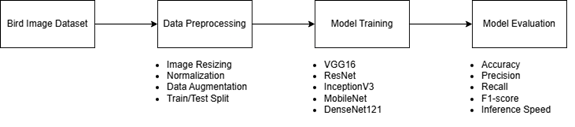
\includegraphics[width=0.9\linewidth]{images/training_pipeline.png}
    \caption{Overview of the model training and evaluation pipeline}
    \label{fig:training_pipeline}
\end{figure}

Each selected architecture was initialized with pretrained ImageNet weights.
This is a common practice in similar bird species classification studies
\cite{bilgin2022bird,tang2025comparative,lolge2025evolution}. Transfer
learning significantly reduces training time and improves model convergence,
especially when working with limited computational resources. The original
classification layers of each model were replaced with new fully connected
layers corresponding to the number of bird species included in the dataset.

Training was performed in two phases. In the first phase, the pretrained backbone layers were
frozen and only the newly added classification layers were trained. In the second phase, all
layers were unfrozen and the entire network was fine-tuned using differential learning rates.
A smaller learning rate was applied to the pretrained backbone layers, while a higher learning
rate was used for the classifier layers.

Images were preprocessed using resizing and normalization techniques. 
Random resized cropping, horizontal flipping, and color jittering were also applied to
the training images in order to improve generalization performance of models and reduce overfitting.

Supervised learning was used during model training. Input images and their
corresponding species labels were provided to the models in batches. During
forward propagation, the models generated predicted class probabilities for
each input image. The cross-entropy loss function was used because the task 
involved multi-class image classification. Model parameters were updated using 
the backpropagation algorithm together with the Adam optimization algorithm.

Training was performed for a predefined maximum number of epochs. A cosine annealing
learning rate scheduler was used to gradually reduce the learning rate during training.
Additionally, gradient clipping was applied to improve training stability. Validation loss and
accuracy values were recorded after each epoch, and validation performance was continuously
monitored to detect potential overfitting. Early stopping was employed during the fine-tuning
phase to terminate training when validation loss stopped improving for a predefined number
of epochs.

Model checkpoints were automatically saved whenever validation accuracy improved. This
ensured that the best-performing versions of the models were preserved for evaluation.

To ensure a fair comparison between architectures, the same dataset splits
were used for all experiments. Batch sizes were selected according to the memory requirements of each architecture.
The models were then evaluated using consistent evaluation metrics, and all
experimental settings and configurations were documented to ensure reproducibility.
The main training hyperparameters used for each model are summarized in
Table~\ref{tab:training_hyperparameters}.

\begin{table}[H]
\centering
\caption{Training Hyperparameters Used for Each Model}
\label{tab:training_hyperparameters}
\begin{tabular}{lccccc}
\hline
Model & Batch Size & Freeze Epochs & Fine-tune Epochs & Head LR & Backbone LR \\
\hline
MobileNetV2 & 32 & 5 & 20 & $10^{-3}$ & $10^{-5}$ \\
ResNet50 & 16 & 5 & 20 & $10^{-3}$ & $10^{-5}$ \\
DenseNet121 & 16 & 5 & 20 & $10^{-3}$ & $10^{-5}$ \\
InceptionV3 & 16 & 5 & 20 & $10^{-3}$ & $10^{-5}$ \\
VGG16 & 8 & 10 & 20 & $10^{-3}$ & $10^{-5}$ \\
\hline
\end{tabular}
\end{table}

\subsubsection{Model Evaluation}

\paragraph{Evaluation Metrics:}

\paragraph{Evaluation Process:}

\subsubsection{=== TODO fine tuning}

\subsection{Web Platform Development}

\subsubsection{Backend Development}

\subsubsection{Database Design}

\subsubsection{Frontend Development}

\subsubsection{Map Integration}

\subsubsection{Development Tools}

\subsubsection{Machine Learning Model Integration}

\clearpage